\documentclass{article}

\usepackage[english]{babel}
\usepackage{gensymb}
\usepackage[letterpaper,top=1.5cm,bottom=1.5cm,left=2cm,right=3cm,marginparwidth=1.5cm]{geometry}
\usepackage{listings}
\usepackage{graphicx}

% Useful packages
\usepackage{amsmath}
\usepackage{graphicx}
\usepackage[colorlinks=true, allcolors=blue]{hyperref}

\title{Report Advanced Programming for HPC}
\author{Ha Ngoc Linh - M21.ICT006}

\begin{document}
\maketitle

\section{Formula}
\subsection{RGB to HSV}
\begin{equation}
H = \begin{cases}
0 \degree &\text{ $\Delta\ =  0$}\\
60 \degree \times \frac{G - B}{\Delta}mod 6 &\text{ $max\ =  R$}\\
60 \degree \times \frac{B - R}{\Delta} + 2 &\text{ $max\ =  G$}\\
60 \degree \times \frac{R - G}{\Delta} + 4 &\text{ $max\ =  B$}\\
\end{cases}
\end{equation}

\begin{equation}
S = \begin{cases}
0  &\text{ $\max =  0$}\\
\frac{\Delta}{max} &\text{ $max\ \neq  0$}\\
\end{cases}
\end{equation}

\begin{equation}
V = max
\end{equation}

\subsection{Kuwahara filter}

\begin{enumerate}

\item Get V value in HSV space of the image.
\item Define window size (region size) ({\omega}).

\item In each region:

    \begin{itemize}
    
        \item Calculate the summary value of all pixels in the region to get the mean value 
        \begin{equation}
            mean = \frac{\sum r(x,y)}{\omega \times \omega}
        \end{equation}
        \item Calculate the standard deviation of the region i
        \begin{equation}
            std_i = \sqrt{\frac{\sum ((V(x,y) - mean)^2)}{\omega \times \omega}}
        \end{equation}
    
    \end{itemize}

\item Find the minimum value in 4 standard deviation values (4 regions)

\item Assign mean(R,G,B) value of this region as new color
    \begin{equation}
        R = avg_R = \frac{\sum(R(x,y)}{\omega \times \omega}
    \end{equation}
    \begin{equation}
        B = avg_B = \frac{\sum(B(x,y)}{\omega \times \omega}
    \end{equation}
    \begin{equation}
        G = avg_G = \frac{\sum(G(x,y)}{\omega \times \omega}
    \end{equation}

\end{itemize}

\end{enumerate}

\section{Kuwahara filter in CPU}

\subsection{Transfer RGB to HSV in CPU}

To transfer RGB to HSV, I follow the formula (1), (2), (3) on each pixel of the image:
\begin{lstlisting}[language=Python]
    height, width = src.shape[0], src.shape[1]
    for tidx in range(height):
       for tidy in range(width):
\end{lstlisting}
I calculate H, S, V values of each pixel by following this code:
\begin{lstlisting}[language=Python]
            b = src[tidx, tidy, 0] / 255
            g = src[tidx, tidy, 1] / 255
            r = src[tidx, tidy, 2] / 255
            cmax = max(r, g, b)
            cmin = min(r, g, b)
            delta = cmax - cmin
            if delta == 0:
                h = 0
            elif cmax == r:
                h = ((((g - b) / delta) % 6) * 60)  % 360
            elif cmax == g:
                h = ((((b - r) / delta) + 2) * 60) % 360
            elif cmax == b:
                h = ((((r - g) / delta) + 4) * 60) % 360
            if cmax == 0:
                s = 0
            else:
                s = delta / cmax
            v = cmax

            dst[tidx, tidy, 0] = h % 360
            dst[tidx, tidy, 1] = s * 100
            dst[tidx, tidy, 2] = v * 100
\end{lstlisting}

\subsection{Kuwahara filter function in CPU}
Following each step defined in section 1.2
\begin{itemize}
    \item To get V value
    
    \begin{lstlisting}[language=Python]
    v = hsv[:, :, 2]
    \end{lstlisting}

    \item \text{window\_size} will be passed into the Kuwahara filter function with integer type value

    \item On each region, the standard deviation value will be calculated by following code

    \begin{lstlisting}[language=Python]
            # first region  rx1 belongs to [tidx - window_size, tidx] and ry1 belongs to [tidy - window_size, tidy]
            sum1 = np.float32(0)
            for rx1 in range(tidx - window_size, tidx): 
                for ry1 in range(tidy - window_size, tidy): 
                    if rx1 >= 0 and ry1 >= 0 and rx1 < height and ry1 < width:
                        sum1 += v[rx1, ry1]
            # find standard deviation of first region
            mean1 = sum1 / ((window_size) * (window_size))
            sum1 = np.float32(0)
            for rx1 in range(tidx - window_size, tidx): 
                for ry1 in range(tidy - window_size, tidy): 
                    if rx1 >= 0 and ry1 >= 0 and rx1 < height and ry1 < width:
                        sum1 += (v[rx1, ry1] - mean1) ** 2
            std1 = math.sqrt(sum1 / ((window_size) * (window_size)))
    \end{lstlisting}

    The calculation is the same for 3 regions left by looping all the pixels of the image
    
    \begin{lstlisting}[language=Python]
    height, width = src.shape[0], src.shape[1]
    for tidx in range(height):
        for tidy in range(width):
    \end{lstlisting}

    \item finding the minimum standard deviation value
    
    \begin{lstlisting}[language=Python]
    min_std = min(std1, std2, std3, std4)
    \end{lstlisting}

    \item Calculate the mean of RGB space color of the region as new color

    \begin{lstlisting}[language=Python]
            # assign the mean of the region with minimum standard deviation to the pixel
            avg_r = np.float32(0)
            avg_g = np.float32(0)
            avg_b = np.float32(0)

            if min_std == std1:
                for rx1 in range(tidx - window_size, tidx): 
                    for ry1 in range(tidy - window_size, tidy): 
                        if rx1 >= 0 and ry1 >= 0 and rx1 < height and ry1 < width:
                            avg_r += src[rx1, ry1, 2]
                            avg_g += src[rx1, ry1, 1]
                            avg_b += src[rx1, ry1, 0]
            if min_std == std2:
                for rx2 in range(tidx, tidx + window_size): 
                    for ry2 in range(tidy - window_size, tidy): 
                        if rx2 >= 0 and ry2 >= 0 and rx2 < height and ry2 < width:
                            avg_r += src[rx2, ry2, 2]
                            avg_g += src[rx2, ry2, 1]
                            avg_b += src[rx2, ry2, 0]

            if min_std == std3:
                for rx3 in range(tidx - window_size, tidx): 
                    for ry3 in range(tidy, tidy + window_size): 
                        if rx3 >= 0 and ry3 >= 0 and rx3 < height and ry3 < width:
                            avg_r += src[rx3, ry3, 2]
                            avg_g += src[rx3, ry3, 1]
                            avg_b += src[rx3, ry3, 0]

            if min_std == std4:
                for rx4 in range(tidx, tidx + window_size): 
                    for ry4 in range(tidy, tidy + window_size): 
                        if rx4 >= 0 and ry4 >= 0 and rx4 < height and ry4 < width:
                            avg_r += src[rx4, ry4, 2]
                            avg_g += src[rx4, ry4, 1]
                            avg_b += src[rx4, ry4, 0]

            avg_r = avg_r / (window_size * window_size)
            avg_g = avg_g / (window_size * window_size)
            avg_b = avg_b / (window_size * window_size)

            dst[tidx, tidy, 2] = avg_r
            dst[tidx, tidy, 1] = avg_g
            dst[tidx, tidy, 0] = avg_b
    \end{lstlisting}
    
\end{itemize}
\newpage
\section{Kuwahara filter in GPU}

\subsection{RGB to HSV in GPU}
With the same formula (1), (2), (3) but using GPU
Instead of using for loop, cuda will be used for processing 

    \begin{lstlisting}[language=Python]
    tidx = cuda.threadIdx.x + cuda.blockIdx.x * cuda.blockDim.x
    tidy = cuda.threadIdx.y + cuda.blockIdx.y * cuda.blockDim.y
    \end{lstlisting}
The formula is the same as the CPU function so in GPU, there is no much different in this part

    \begin{lstlisting}[language=Python]
    b = src[tidx, tidy, 0] / 255
    g = src[tidx, tidy, 1] / 255
    r = src[tidx, tidy, 2] / 255
    cmax = max(r, g, b)
    cmin = min(r, g, b)
    delta = cmax - cmin
    if delta == 0:
        h = 0
    elif cmax == r:
        h = ((((g - b) / delta) % 6) * 60)  % 360
    elif cmax == g:
        h = ((((b - r) / delta) + 2) * 60) % 360
    elif cmax == b:
        h = ((((r - g) / delta) + 4) * 60) % 360
    if cmax == 0:
        s = 0
    else:
        s = delta / cmax
    v = cmax

    dst[tidx, tidy, 0] = h % 360
    dst[tidx, tidy, 1] = s * 100
    dst[tidx, tidy, 2] = v * 100
    \end{lstlisting}

\subsection{Kuwahara filter in GPU without shared memory}
With the same formula (4), (5), (6), (7), (8) of using-CPU function, the code for processing filtering Kuwahara with GPU is not much different from using CPU
The first step is getting V value from the image in HSV space. This step is not different from the CPU function
Instead of using loop, by using cuda, we have:
    \begin{lstlisting}[language=Python]
    tidx = cuda.threadIdx.x + cuda.blockIdx.x * cuda.blockDim.x
    tidy = cuda.threadIdx.y + cuda.blockIdx.y * cuda.blockDim.y
    \end{lstlisting}
The process on each region is not different from the CPU function. (The code is the same as the section 2.2)

\subsection{Kuwahara filter in GPU with shared memory}
\newpage
\section{Comparing Kuwahara function between using CPU and GPU}

Using the same image to apply Kuwahara filter in both CPU and GPU:

    \begin{figure}
        \centering
        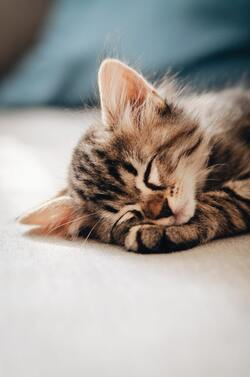
\includegraphics{cute-cat.jpg}
        \caption{original image}
        \label{fig:figure1}
    \end{figure}

Apply Kuwahara filter with CPU function: (the timer is added to get the running time)

    \begin{lstlisting}[language=Python]
    # start timer
    start = time.time()
    filtered = kuwahara_filter_hsv(root, v, 8)
    # end timer
    end = time.time()
    print("Time taken for kuwahara filter in CPU: ", end - start)
    \end{lstlisting}

Apply Kuwahara filter with GPU function: (the timer is added to get the running time)

    \begin{lstlisting}[language=Python]
    blockSize = (16, 16)
    gridSize = (math.ceil(gpu_img.shape[0] / blockSize[0]), math.ceil(gpu_img.shape[1] / blockSize[1]))
    output_cuda_image_data = cuda.device_array(np.shape(gpu_img), np.uint8)
    # start timer
    start = time.time()
    kuwahara_filter_hsv[gridSize, blockSize](gpu_img, output_cuda_image_data, v, 8)
    # end timer
    end = time.time()
    print("Time taken for kuwahara in GPU: ", end - start)
    \end{lstlisting}

    In both function, the window\_size was be assigned by 8

    The result of 2 functions :

    \begin{figure}
        \centering
        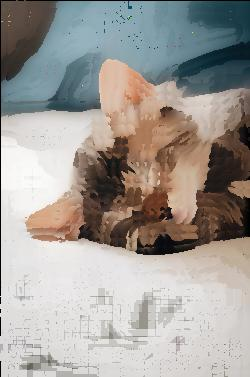
\includegraphics{cute-cat-kuwahara_cpu.jpg}
        \caption{Kuwahara filter in CPU}
        \label{fig:figure2}
    \end{figure}

    \begin{figure}
        \centering
        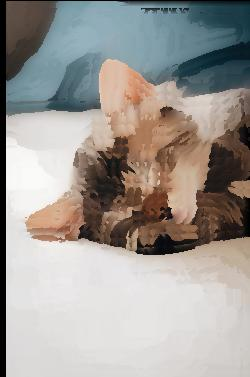
\includegraphics{cute-cat-kuwahara_gpu.jpg}
        \caption{Kuwahara filter in GPU}
        \label{fig:figure3}
    \end{figure}

    There is a little bit difference between 2 output images. The reason may come from variable type and how I detect the position of each region

    The running time of each functions are:

    \begin{itemize}
        \item CPU: 87.74110865592957s
        \item GPU: 1.6664512157440186s
    \end{itemize}

    
    The running time is affected by the size of the image 
    (in this case, the image size is 250*377  and the file size is 14,486 bytes). In this test, I run the on google Colab free version.
    But it is clear to see that in GPU, the performance is much better than CPU
    
\end{document}